\chapter{The Two Technologies}
\label{ch:methods}

The problem set in Section~\ref{sec:problem-set} asks for one system and names two technologies inside it. This chapter specifies both of them at the level a second implementation could follow. Section~\ref{sec:rch} specifies resource-coupled heterogeneous graph attention scheduling: the objectives, the resource constraints, the graph, the attention score, the masked policy, and the way that policy is trained. Section~\ref{sec:ssdt} specifies the status-synchronized digital twin: the health dynamics, the revision of health from a noisy reading, the chance constraint, the preventive-maintenance action, and the write-back of the renewed health into the graph of Section~\ref{sec:rch}. Each section ends with the same numerical assignment, a navy backpack shell on the two cutters, so that the formulas are not left as symbols only.

The estimation in Chapter~\ref{ch:estimation} uses a one-hop executable form of the score and a hazard form of the chance constraint. Those forms are stated here as the operational model. The multi-layer network and the Kalman revision are stated as the plant model one would run when real sensor streams, rather than a simulator that already knows its own wear, are the source of \(h_k\).

\section{Resource-coupled heterogeneous graph attention}
\label{sec:rch}

\subsection{Sets, routes, and the decision that is actually taken}

Let \(J\) be the set of released orders and \(M\) the set of machines. Each order \(j \in J\) has a release time \(r_j\), a due date \(d_j\), a colour \(c_j\), a size, a quantity \(q_j\), and an ordered route of operations \(O_{1j},\ldots,O_{n_j j}\). Operation \(O_{ij}\) has a base duration \(\tau_{ij}\) defined at the reference quantity \(q_0 = 80\) and reference size M, an eligible set of machine groups \(G_{ij}\), and a token type \(u_{ij} \in \{\mathrm{die},\mathrm{colour},\mathrm{none}\}\).

Let \(K\) be the set of operators. Operator \(o\) has a skill \(\sigma_{ok} > 0\) only for the machine groups that person is allowed to run, and \(\sigma_{ok} = 0\) otherwise. Let \(Q\) be the set of token pools. The die pool has capacity \(n_{\mathrm{die}}\). The colour pool of colour \(c\) has capacity \(n_c\). A pool of capacity zero would make every operation of that colour infeasible; the factory data do not contain such a pool.

A dispatch at time \(t\) is a bundle
\begin{equation}
a = (i,j,k,o) ,
\label{eq:bundle}
\end{equation}
meaning that operation \(O_{ij}\) starts on machine \(k\) with operator \(o\). If \(u_{ij}\) is a die or a colour, the bundle also seizes one unit of that pool for the whole occupation of the machine. The bundle is the action of the policy. It is larger than the operation-machine pair of Song, Chen, Li, and Cao \cite{song2023}, and the extra components are the reason the graph in this section has more than two node types.

\subsection{Objectives}

A complete schedule \(S\) is the set of bundles that were started, together with the clock times at which they started and finished. Five functions of \(S\) are kept separate until a preference vector combines them. The makespan is
\begin{equation}
f_1(S) = \cmax = \max_{j \in J} C_j .
\label{eq:f1}
\end{equation}
Total tardiness is
\begin{equation}
f_2(S) = \sum_{j \in J} \max(0, C_j - d_j) .
\label{eq:f2}
\end{equation}
Energy sums every occupation, including setup minutes and preventive-maintenance minutes, and adds the expected energy of an interruption,
\begin{equation}
f_3(S) = \sum_{a \in S} P_k \frac{\Delta_a}{60}\big(1 + \gamma_E h_k\big) + \sum_{a \in S} \phi_a \, P_k^{\mathrm{rep}} \frac{\Delta^{\mathrm{rep}}}{60}\big(1 + \gamma_E h_k\big) .
\label{eq:f3}
\end{equation}
Here \(P_k\) is the nameplate power of machine \(k\) in kilowatts, \(\Delta_a\) is the occupation in minutes, \(h_k\) is the health used for that occupation, \(\gamma_E = 0.45\) is the wear surcharge on power, \(\phi_a\) is the failure probability of the cycle, and the repair term uses half the nameplate power for \(\Delta^{\mathrm{rep}} = 48\) minutes. The half-power repair is a modelling choice: a stopped head does not cut, but the drive and the recovery move are not free.

Workload imbalance is the standard deviation of busy minutes,
\begin{equation}
f_4(S) = \left(\frac{1}{|M|}\sum_{k \in M}\big(B_k - \bar B\big)^2\right)^{1/2}, \qquad B_k = \sum_{a:\,k(a)=k} \Delta_a .
\label{eq:f4}
\end{equation}
Expected failures are the sum of the cycle probabilities,
\begin{equation}
f_5(S) = \sum_{a \in S} \phi_a .
\label{eq:f5}
\end{equation}
A preference \(\omega \in \R^4\) with \(\omega \ge 0\) and \(\sum_{m=1}^{4}\omega_m = 1\) defines the scalar that a single policy optimises,
\begin{equation}
J_\omega(S) = \sum_{m=1}^{4} \omega_m \, \tilde f_m(S) + \lambda_\Phi \, \tilde f_5(S) ,
\label{eq:scalar}
\end{equation}
where a tilde denotes division by the same function evaluated on the first-in-first-out schedule of the same order book. The ratio keeps a minute of makespan from being added to a kilowatt-hour. The failure term keeps a weight \(\lambda_\Phi\) even when the manager's four-way preference does not mention breakdowns, because a schedule that fails machines is not an admissible way to win the other four numbers. In the estimation, \(\lambda_\Phi = 0.12\) during identification and the reported tables always show the five raw functions, not only \(J_\omega\).

Equation~\eqref{eq:scalar} is a scalarisation, not a claim that the five functions have a single optimum. Changing \(\omega\) is how the factory moves along the conflicts described in Section~\ref{sec:problem-set}. NSGA-II remains available as an offline reference precisely because a scalarisation can miss a region of the front \cite{deb2002}. The online system is allowed to be a scalarisation because the dispatch decision cannot wait for a front.

\subsection{Constraints}

Let \(x_{ijko} \in \{0,1\}\) be one when bundle \((i,j,k,o)\) is the bundle that executes \(O_{ij}\). Every operation is executed once,
\begin{equation}
\sum_{k \in M_{ij}} \sum_{o \in K_{ij}} x_{ijko} = 1 ,
\label{eq:assign-once}
\end{equation}
where \(M_{ij} = \{k : \mathrm{group}(k) \in G_{ij}\}\) and \(K_{ij}\) is the set of operators with positive skill on the chosen machine. Precedence inside the route is
\begin{equation}
S_{i+1,j} \ge C_{ij} , \qquad C_{ij} = S_{ij} + \Delta_{ij} ,
\label{eq:precedence}
\end{equation}
and the release date is \(S_{1j} \ge r_j\).

Machine capacity and operator capacity are disjunctive. For any two distinct occupations of the same machine, one finishes before the other starts, and the same statement holds for an operator. With a binary order variable \(y\),
\begin{equation}
C_{a} \le S_{a'} + H(1-y_{aa'}) , \qquad C_{a'} \le S_{a} + H y_{aa'} ,
\label{eq:disjunct}
\end{equation}
for a horizon constant \(H\) large enough to dominate any feasible day. Token capacity is a knapsack at every time. For the die pool, and likewise for each colour with its own capacity,
\begin{equation}
\sum_{a \in A(t)} \1\{u_a = \mathrm{die}\} \le n_{\mathrm{die}} ,
\label{eq:token}
\end{equation}
where \(A(t)\) is the set of occupations that cover time \(t\). Skill is a hard mask rather than a penalty: \(x_{ijko} = 0\) whenever \(\sigma_{o,\mathrm{group}(k)} = 0\).

Setups are sequence dependent on colour. If machine \(k\) has just run colour \(c\) and the next occupation has colour \(c_j \ne c\), a setup of \(s^{\mathrm{col}} = 11\) minutes is inserted before processing. The first occupation of a colour-sensitive machine after a cleared state pays a warm-up of \(s^{\mathrm{warm}} = 4\) minutes. Hardware, inspection, and packing do not pay a colour setup. The setup occupies both the machine and the operator, and it occupies the token, because the die or the thread is the thing being changed.

These constraints are the integer program a solver would be given if the health state were frozen and no new order could appear. The shop does not offer those two favours. Health is a function of the schedule, so \(\Delta_{ij}\) depends on a state that the binaries themselves change, and orders appear at release dates the morning plan does not know. The integer program is the definition of feasibility. The policy below is the object that constructs a feasible \(x\) online.

\subsection{Processing time at a given health}

The duration of the processing part of a bundle, before setup and before any maintenance, is
\begin{equation}
p_{ijko}(h_k) = \tau_{ij}\,\frac{q_j}{q_0}\,\zeta_j\,\frac{1 + \alpha h_k^{\beta}}{v_k \, \sigma_{ok}} .
\label{eq:ptime}
\end{equation}
The quantity ratio \(q_j/q_0\) and the size factor \(\zeta_j \in \{0.88, 1.00, 1.16\}\) scale the batch. The machine speed \(v_k\) and the operator skill \(\sigma_{ok}\) scale the rate. The factor \(1 + \alpha h_k^{\beta}\) is the status effect, with \(\alpha = 0.85\) and \(\beta = 1.15\). The exponent above one makes the last part of the wear more expensive than the first, which is the empirical shape of a knife and of a needle that has started to heat. At \(h_k = 0\) the factor is one and the formula collapses to an ordinary flexible-job-shop time. At the health values used in the case, the factor is about \(1.45\) on the worn automatic cutter and about \(1.15\) on the healthy manual cutter. Those two numbers are computed in the worked example at the end of this section.

Equation~\eqref{eq:ptime} is the first place the twin enters the scheduler. A policy that treats \(p\) as a constant stored in a routing table is using \(\alpha = 0\), whether or not a screen on the wall shows \(h_k\).

\subsection{The heterogeneous graph of one decision}

At time \(t\) the ready set \(R(t)\) contains every operation whose predecessor in the same order is finished and whose order has been released. A candidate is a triple \((O_{ij}, k, o)\) with \(O_{ij} \in R(t)\), machine \(k\) eligible and free, operator \(o\) skilled and free, and the required token available. Candidates that fail any of those tests are not scored. Masking them is part of the model, not a cleanup after the network.

Each candidate induces a four-node heterogeneous graph. The operation node carries the time and due-date pressure of this bundle. The machine node carries health, load, energy, and failure. The operator node carries the skill gap. The shop node carries contention for the colour, the die, and the machine group. Edges are typed. A precedence edge is not drawn inside the candidate graph, because precedence has already been enforced by membership of \(R(t)\). The typed edges that remain are eligibility (operation--machine), assignment (operation--operator), seizure (operation--token, summarised on the shop node), and context (each node--shop). Figure~\ref{fig:rch-graph} draws one candidate.

\begin{figure}[ht]
\centering
\begin{tikzpicture}[
  n/.style={draw, circle, minimum size=1.15cm, font=\small, align=center},
  arr/.style={-{Stealth}, thick}
]
\node[n] (op) {op};
\node[n, right=2.2cm of op] (m) {machine};
\node[n, below=1.5cm of op] (o) {operator};
\node[n, below=1.5cm of m] (s) {shop};
\draw[arr] (op) -- node[above, font=\scriptsize] {eligible} (m);
\draw[arr] (op) -- node[left, font=\scriptsize] {skill} (o);
\draw[arr] (m) -- node[right, font=\scriptsize] {load} (s);
\draw[arr] (o) -- node[below, font=\scriptsize] {pool} (s);
\draw[arr] (op) -- node[above, font=\scriptsize, sloped] {token} (s);
\end{tikzpicture}
\caption{One-hop heterogeneous graph of a single candidate bundle. The full shop graph is the union of these candidate graphs at the current ready set. Attention pools the four nodes; it does not mix two candidates before the scores are compared.}
\label{fig:rch-graph}
\end{figure}

The twelve raw costs of a candidate, all scaled to lie near the unit interval, are
\begin{align}
\rho_1 &= p/45, &
\rho_2 &= s/11, &
\rho_3 &= \max(0,-\ell)/180, \label{eq:raw1}\\
\rho_4 &= (p + W)/ \max(30, d_j - t), &
\rho_5 &= h_k, &
\rho_6 &= \max(0, B_k - \bar B)/80, \label{eq:raw2}\\
\rho_7 &= E_{\mathrm{cycle}}, &
\rho_8 &= \phi, &
\rho_9 &= n^{\mathrm{col}} / n_{c_j}, \label{eq:raw3}\\
\rho_{10} &= n^{\mathrm{die}} / n_{\mathrm{die}}, &
\rho_{11} &= n^{\mathrm{group}}/3, &
\rho_{12} &= \max(0, 1.05 - \sigma_{ok}) . \label{eq:raw4}
\end{align}
Slack \(\ell\) is the due date minus the earliest plausible completion of the rest of the route. \(W\) is the base work remaining after this operation. The three contention counts \(n^{\mathrm{col}}\), \(n^{\mathrm{die}}\), and \(n^{\mathrm{group}}\) are the numbers of ready operations that want the same colour lot, the die pool, or the same machine group. They are the graph readout of the shop node: a mean, over neighbours, of demand. A candidate that looks short on \(\rho_1\) and disastrous on \(\rho_9\) is a khaki body started while two other khaki bodies are already waiting for the single lot.

The four node keys collapse the twelve costs along the node types,
\begin{align}
\kappa_{\mathrm{op}} &= \rho_1 + \rho_2 + 1.4\rho_3 + \rho_4 , \label{eq:key-op}\\
\kappa_{\mathrm{m}} &= \rho_5 + \rho_6 + 0.35\rho_7 + 1.6\rho_8 , \label{eq:key-m}\\
\kappa_{\mathrm{o}} &= \rho_{12} + 0.3\rho_{11} , \label{eq:key-o}\\
\kappa_{\mathrm{s}} &= \rho_9 + \rho_{10} + 0.5\rho_{11} . \label{eq:key-s}
\end{align}
Positive learned weights \(w_1,\ldots,w_{12}\) form the node costs
\begin{align}
c_{\mathrm{op}} &= w_1\rho_1 + w_2\rho_2 + w_3\rho_3 + w_4\rho_4 , \label{eq:node-op}\\
c_{\mathrm{m}} &= w_5\rho_5 + w_6\rho_6 + w_7\rho_7 + w_8\rho_8 , \label{eq:node-m}\\
c_{\mathrm{o}} &= w_{12}\rho_{12} , \label{eq:node-o}\\
c_{\mathrm{s}} &= w_8'\rho_9 + w_9\rho_{10} + w_{10}\rho_{11} , \label{eq:node-s}
\end{align}
where the shop-node weights are \(w_8, w_9, w_{10}\) in the parameter vector (the prime in \eqref{eq:node-s} is only there to keep the failure weight \(w_8\) of \eqref{eq:node-m} visually distinct; the implementation stores twelve weights and does not share them). Positivity is obtained by storing the logarithm and exponentiating, so a coordinate descent cannot flip a cost into a reward by accident.

\subsection{Attention and the preference}

Let \(a_{\mathrm{op}}, a_{\mathrm{m}}, a_{\mathrm{o}}, a_{\mathrm{s}}\) be attention biases and let \(g \in \R^4\) be a gate vector. The preference opens each node by
\begin{align}
\pi_{\mathrm{op}} &= 0.55 + g_1(\omega_1 + \omega_2) , \label{eq:open-op}\\
\pi_{\mathrm{m}} &= 0.55 + g_2(\omega_3 + 0.5\omega_1) , \label{eq:open-m}\\
\pi_{\mathrm{o}} &= 0.45 + g_3 \omega_4 , \label{eq:open-o}\\
\pi_{\mathrm{s}} &= 0.45 + g_4(\omega_2 + 0.25) . \label{eq:open-s}
\end{align}
Time and due-date weight open the operation node. Energy, and part of the makespan weight, open the machine node, because health and failure destroy makespan as well as kilowatt-hours. Balance opens the operator node. Due-date weight also opens the shop node, because token contention is how a due date is missed when the machine itself is free. The attention weights are a softmax over the opened keys,
\begin{equation}
\alpha_u = \frac{\exp(a_u + \pi_u \kappa_u)}{\sum_{u' \in \{\mathrm{op,m,o,s}\}} \exp(a_{u'} + \pi_{u'} \kappa_{u'})} .
\label{eq:alpha}
\end{equation}
The candidate score, which the policy minimises, is the opened, attention-weighted node cost
\begin{equation}
\psi(a) = \sum_u \alpha_u \, \pi_u \, c_u .
\label{eq:psi}
\end{equation}
Equation~\eqref{eq:alpha} is one-head, one-hop graph attention \cite{velickovic2018}. It is the operational policy. The multi-layer form used as the scalable model replaces the hand-grouped keys by learned maps. For each relation \(r\) and layer \(\ell\),
\begin{equation}
e_{uv}^{(r,\ell)} = \mathrm{LeakyReLU}\!\left(b_r^{\top}\big[W_r^{(\ell)} z_u^{(\ell)} \,\|\, W_r^{(\ell)} z_v^{(\ell)}\big]\right) ,
\label{eq:gat-full}
\end{equation}
\begin{equation}
\alpha_{uv}^{(r,\ell)} = \frac{\exp(e_{uv}^{(r,\ell)})}{\sum_{v' \in N_r(u)} \exp(e_{uv'}^{(r,\ell)})} ,
\qquad
z_u^{(\ell+1)} = \sigma\!\left(\sum_r \sum_{v \in N_r(u)} \alpha_{uv}^{(r,\ell)} W_r^{(\ell)} z_v^{(\ell)}\right) .
\label{eq:gat-update}
\end{equation}
The candidate score of the full model is a linear map of the concatenated final embeddings of the four nodes, again gated by \(\omega\). Equation~\eqref{eq:psi} is what Chapter~\ref{ch:estimation} runs. Equations~\eqref{eq:gat-full} and \eqref{eq:gat-update} are what a larger plant would train with the proximal policy method below, once more than a few dozen order books exist as logged transitions. Both are the same technology: a preference-conditioned attention pool over a resource-typed graph, followed by a masked choice of bundle.

\subsection{Markov decision process}

The dispatch process is a Markov decision process \(( \mathcal{S}, \mathcal{A}, P, R, \gamma )\). A state \(s_t \in \mathcal{S}\) contains the ready set, the free times and previous colours of machines and operators, the residual token capacities, the health vector, and the preference \(\omega\). An action \(a_t\) is a feasible bundle, or a bundle preceded by preventive maintenance when Section~\ref{sec:ssdt} says so. The transition \(P\) advances the clock to the next moment at which a machine and an operator are free, releases tokens of finished work, inserts any order whose release time has arrived, and updates health by the wear map of Section~\ref{sec:ssdt}. The reward is the change in the scalar cost. With \(J_\omega\) evaluated on the partial schedule,
\begin{equation}
r_t = -\big( J_\omega(S_{t+1}) - J_\omega(S_t) \big) ,
\label{eq:reward}
\end{equation}
so that a step which lengthens the day, the tardiness, the energy, the imbalance, or the failure sum returns a negative reward. The discount \(\gamma \in (0,1)\) is kept close to one because a setup avoided now pays its tardiness much later. The estimation identifies coefficients by the total \(J_\omega\) of the finished day, which is the undiscounted, finite-horizon form of the same objective.

The policy \(\pi_\theta(a \mid s, \omega)\) is a softmax over the negative scores of the feasible candidates,
\begin{equation}
\pi_\theta(a \mid s, \omega) = \frac{\exp(-\psi_\theta(a)/\tau)}{\sum_{a' \in \mathcal{F}(s)} \exp(-\psi_\theta(a')/\tau)} ,
\label{eq:policy}
\end{equation}
where \(\mathcal{F}(s)\) is the masked feasible set and \(\tau\) is a temperature. At execution, \(\tau \to 0\) and the policy takes the minimiser of \(\psi\). During stochastic training, a positive temperature supplies the exploration that a cross-entropy search gets instead from its sampling distribution.

\subsection{Training the full model with proximal policy optimisation}

The full model is trained by proximal policy optimisation \cite{schulman2017}. Let \(\theta\) collect the maps \(W_r\), the attention vectors, the gates, and the value-function weights. Along a trajectory the probability ratio of a new policy to the policy that collected the data is
\begin{equation}
\eta_t(\theta) = \frac{\pi_\theta(a_t \mid s_t, \omega)}{\pi_{\theta_{\mathrm{old}}}(a_t \mid s_t, \omega)} .
\label{eq:ratio}
\end{equation}
The clipped surrogate is
\begin{equation}
L^{\mathrm{clip}}(\theta) = \E_t \Big[ \min\big( \eta_t(\theta) \hat A_t,\; \mathrm{clip}(\eta_t(\theta), 1-\epsilon, 1+\epsilon)\, \hat A_t \big) \Big] ,
\label{eq:ppo}
\end{equation}
with \(\epsilon\) typically \(0.2\). The advantage \(\hat A_t\) is the generalised advantage estimate of the scalar reward \eqref{eq:reward}. A value head \(V_\phi(s,\omega)\) is trained by squared error against the discounted return, and an entropy bonus \(\beta_H \mathcal{H}(\pi_\theta)\) keeps \eqref{eq:policy} from collapsing to a single bundle before the resource features have been used. The parameter step maximises \(L^{\mathrm{clip}} - c_V L^{\mathrm{value}} + \beta_H \mathcal{H}\).

Preference conditioning is trained by sampling \(\omega\) with each episode, not by training four unrelated networks and hoping their weights happen to be comparable. A single network that has seen many \(\omega\) is what Equation~\eqref{eq:open-op}--\eqref{eq:open-s} approximate when the gates \(g\) are identified at one operating preference and then reused. Chapter~\ref{ch:estimation} is explicit about which of these two regimes the numbers come from: the coefficients were identified at the balanced preference \(\omega = (0.34, 0.33, 0.18, 0.15)\), and the gate formulas were not re-fit for every corner of the simplex. The tolerance sweep of the twin, not the gate formulas, is the knob the estimation shows moving cleanly.

\subsection{Identification used in the estimation system}

The executable score has twenty coefficients: twelve log-weights, four attention biases, and four gates. Direct policy-gradient training of a deep network is not required to identify twenty numbers on a shop of this size, and it would make the tables depend on an optimiser trajectory that a reader cannot see. The estimation therefore uses the cross-entropy method. A Gaussian \(\mathcal{N}(\mu, \mathrm{diag}(\sigma^2))\) proposes a population of coefficient vectors. Each vector is scored by the mean of \(J_\omega\) on a fixed set of training order books, always relative to first-in-first-out on the same book. The elite fraction updates \(\mu\) and \(\sigma\). The search starts from a logarithmic prior that already resembles a blend of shortest processing time, slack, and health, so the first generation is a scheduler rather than a random permutation. Algorithm~\ref{alg:cem} states the loop. The training curve is reported in Chapter~\ref{ch:estimation}.

\begin{algorithm}[ht]
\caption{Cross-entropy identification of the RCH-GAT score}
\label{alg:cem}
\begin{algorithmic}[1]
\State Initialise \(\mu\) from the short-time, slack, and health prior; set \(\sigma \leftarrow 0.35\)
\For{generation \(= 1, \ldots, G\)}
  \For{sample \(= 1, \ldots, N\)}
    \State Draw \(\theta \sim \mathcal{N}(\mu, \mathrm{diag}(\sigma^2))\)
    \State For each training book, run Algorithm~\ref{alg:dispatch} and record \(J_\omega\)
    \State Set the fitness to the mean \(J_\omega\) across the training books
  \EndFor
  \State Keep the elite fraction of \(\theta\)
  \State Set \(\mu\) to their mean and \(\sigma\) to their standard deviation, floored by a small positive constant
\EndFor
\State \Return the elite \(\theta\) with the best fitness observed
\end{algorithmic}
\end{algorithm}

\begin{algorithm}[ht]
\caption{Online dispatch with a masked resource bundle}
\label{alg:dispatch}
\begin{algorithmic}[1]
\State \(t \leftarrow 0\); mark every operation unfinished; set health to the measured \(h_k(0)\)
\While{some operation is unfinished}
  \State Release any order with \(r_j \le t\), and release tokens of occupations that have ended
  \State Build the feasible set \(\mathcal{F}\) of bundles at time \(t\)
  \If{\(\mathcal{F}\) is not empty}
    \State Score each bundle by \eqref{eq:psi}, applying the maintenance test of Algorithm~\ref{alg:ssdt}
    \State Start the minimiser; update free times, colour memory, tokens, health, energy, and \(\phi\)
  \Else
    \State Advance \(t\) to the next completion or the next release
  \EndIf
\EndWhile
\end{algorithmic}
\end{algorithm}

\subsection{What the mask guarantees}

\begin{proposition}
\label{prop:mask}
Suppose every order has a finite route, every operation has at least one eligible machine group, every machine group has at least one operator with positive skill, and every token pool that an operation requires has capacity at least one. Then Algorithm~\ref{alg:dispatch} finishes every released order in finite time, and every started bundle satisfies precedence, machine capacity, operator capacity, and token capacity.
\end{proposition}

\begin{proof}
Every started bundle is taken from \(\mathcal{F}\), and \(\mathcal{F}\) contains only bundles whose predecessor is finished, whose machine and operator are free, whose skill is positive, and whose token pool has a free unit. Capacity and precedence therefore hold by construction of the mask. A started bundle occupies its machine, operator, and token for a finite duration, because base times, size factors, and health factors are finite and health is clipped. At the occupation's end the three resources are released. If \(\mathcal{F}\) is empty and work remains, either a resource is occupied, in which case the clock advances to a release, or an order is unreleased, in which case the clock advances to its release time. The state cannot cycle: each advance of the clock to a completion finishes one operation, and there are finitely many operations. Hence the loop ends with every operation finished.
\end{proof}

The proposition is about feasibility, not about optimality. A first-in-first-out policy satisfies it and still produces the poor tardiness reported in Chapter~\ref{ch:estimation}. The proposition is what makes the comparison in that chapter a comparison of decisions rather than a comparison of repair heuristics. Every method in the estimation, including the classical rules, dispatches through the same mask. They differ only in the score that ranks \(\mathcal{F}\).

\subsection{A numerical assignment without the twin's veto}

Consider one ready operation, the shell cut of a navy backpack, quantity \(80\), size M, so that \(q_j/q_0 = 1\) and \(\zeta_j = 1\). The base time is \(\tau = 24\) minutes. Cutter-A has speed \(v = 1.28\), power \(6.8\,\mathrm{kW}\), wear rate \(0.00115\) per minute, and health \(h = 0.58\). Cutter-B has speed \(0.74\), power \(2.4\,\mathrm{kW}\), and health \(h = 0.22\). Operator Cut-1, with skill \(1\), is free for either machine. No setup is charged in this comparison. Equation~\eqref{eq:ptime} on Cutter-A gives
\begin{equation}
1 + \alpha h^{\beta} = 1 + 0.85 \times 0.58^{1.15} = 1.4543 ,
\end{equation}
\begin{equation}
p_A = 24 \times 1.4543 / 1.28 = 27.268 \ \mathrm{minutes} .
\end{equation}
On Cutter-B,
\begin{equation}
1 + \alpha h^{\beta} = 1 + 0.85 \times 0.22^{1.15} = 1.1490 ,
\end{equation}
\begin{equation}
p_B = 24 \times 1.1490 / 0.74 = 37.265 \ \mathrm{minutes} .
\end{equation}
A shortest-processing-time rule sees \(27.268 < 37.265\) and assigns Cutter-A. The energy of that cycle, from the first term of \eqref{eq:f3} and before the failure term, is
\begin{equation}
E_A = 6.8 \times \frac{27.268}{60} \times (1 + 0.45 \times 0.58) = 3.896\ \mathrm{kWh} ,
\end{equation}
against
\begin{equation}
E_B = 2.4 \times \frac{37.265}{60} \times (1 + 0.45 \times 0.22) = 1.638\ \mathrm{kWh} .
\end{equation}
The fast machine is more than twice as hungry. The failure probability, computed in Section~\ref{sec:ssdt} from the hazard at these health values, is \(0.106\) on A and \(0\) on B. Expected repair delay on A is \(0.106 \times 48 = 5.09\) minutes, so the occupation that shortest processing time thought was \(27.3\) minutes is \(32.4\) minutes once the risk is priced, and it leaves Cutter-A at a predicted health of \(0.58 + 0.00115 \times 27.268 = 0.611\).

The attention score does not have to choose B every time. If the due date is already broken and the other cutter is the bottleneck of a later order, paying \(3.9\,\mathrm{kWh}\) on A can be the lower score under a time-heavy \(\omega\). The point of the numbers is narrower. Any rule that ranks on nominal or even on health-scaled processing time alone will take A. Any score that includes \(\rho_5\), \(\rho_7\), and \(\rho_8\) is allowed to refuse A. That refusal is the resource-and-status content of \(\psi\). Whether the refusal should instead be a sixteen-minute maintenance of A is the twin's decision, made with the same candidate in the next section.

\subsection{Attention arithmetic on the two cutters}

The preceding subsection stopped at the physical times. This one applies the identified score, so that Equation~\eqref{eq:psi} is a number rather than a shape. The coefficient vector is the one stored by Algorithm~\ref{alg:cem} and used for every table in Chapter~\ref{ch:estimation}. Exponentiating the twelve log-weights gives
\begin{equation}
\begin{aligned}
w = (\, &0.288,\ 1.029,\ 0.731,\ 0.235,\ 0.606,\ 5.660,\\
&0.912,\ 1.269,\ 0.133,\ 0.917,\ 0.353,\ 1.657 \,).
\end{aligned}
\label{eq:wstar}
\end{equation}
The order is processing time, setup, slack penalty, critical ratio, health, load deviation, energy, failure probability, colour contention, die contention, group contention, and skill gap. Two facts are already visible. The load weight \(5.660\) is several times any other weight, so a machine that has already run far ahead of its neighbours is expensive even when it is healthy. The colour-contention weight \(0.133\) is the smallest of the twelve, which is the coefficient-level reason the resource ablation in Chapter~\ref{ch:estimation} moves the day only a little.

At the balanced preference \(\omega = (0.34, 0.33, 0.18, 0.15)\) the openings \eqref{eq:open-op}--\eqref{eq:open-s} evaluate to
\begin{equation}
\pi = (1.121,\ 0.908,\ 0.734,\ -0.490).
\label{eq:pi-num}
\end{equation}
The shop-node opening is negative. The identified gate on that node learned to shrink, rather than enlarge, the contention term under this preference. A negative opening does not delete the node. Multiplied into the key, it reduces attention when contention is high; multiplied into the cost, it can even change the sign of that node's contribution. In the cutter arithmetic below the attention mass on the shop node is about \(0.03\), so the sign changes the score by roughly a hundredth. Token pressure is a weak voice, not an inverted one in any way that moves a schedule. That is an empirical outcome of the identification, reported here so that the ablation is not a surprise.

Construct two candidates for the navy shell, both with Cut-1 free, no setup, no slack penalty, and the same token pressure: one other cutting operation is also ready, and the navy pool is half used. Critical ratios are \(0.80\) on A and \(0.95\) on B, because B's longer cycle eats more of the remaining due-date margin. Load deviation is \(0\) on A and \(0.10\) on B. The twelve raw costs are then
\begin{align}
\rho^{A} &= (0.606,\ 0,\ 0,\ 0.800,\ 0.580,\ 0,\ 3.896,\ 0.106,\ 0.500,\ 0.500,\ 0.667,\ 0), \\
\rho^{B} &= (0.828,\ 0,\ 0,\ 0.950,\ 0.220,\ 0.100,\ 1.638,\ 0,\ 0.500,\ 0.500,\ 0.667,\ 0).
\end{align}
Node keys and node costs follow \eqref{eq:key-op}--\eqref{eq:node-s}. For Cutter-A,
\begin{equation}
\kappa^{A} = (1.406,\ 2.113,\ 0.200,\ 1.333), \qquad
c^{A} = (0.363,\ 4.038,\ 0,\ 0.760).
\end{equation}
The machine-node cost \(4.038\) is almost entirely energy: \(0.912 \times 3.896 = 3.55\), with health and failure making up the rest. For Cutter-B,
\begin{equation}
\kappa^{B} = (1.778,\ 0.893,\ 0.200,\ 1.333), \qquad
c^{B} = (0.462,\ 2.193,\ 0,\ 0.760).
\end{equation}
Softmax attention \eqref{eq:alpha} with the biases \(a = (1.082, 0.969, -0.707, 0.672)\) puts mass
\begin{equation}
\alpha^{A} = (0.422,\ 0.531,\ 0.017,\ 0.030), \qquad
\alpha^{B} = (0.742,\ 0.203,\ 0.020,\ 0.035).
\end{equation}
On the worn cutter, attention sits on the machine node, because that node's key is large. On the healthy cutter, attention sits on the operation node, because the machine key has collapsed. The scores are
\begin{equation}
\psi(A) = 2.108, \qquad \psi(B) = 0.776.
\end{equation}
The policy takes B. Shortest processing time, using \(27.3 < 37.3\), takes A. The difference is not a hidden rule. It is the machine-node cost of \(6.8\,\mathrm{kW}\) at health \(0.58\), amplified by an attention weight of \(0.531\).

Table~\ref{tab:weights} is the same vector, written so a reader can see which physical effect survived identification.

\begin{table}[ht]
\centering
\caption{Identified positive weights on the twelve costs, from \eqref{eq:wstar}. A large weight means the identification was willing to avoid that cost even when other costs rose.}
\label{tab:weights}
\small
\begin{tabular}{lrll}
\toprule
Cost & Weight & Node & What a large value punishes \\
\midrule
Processing time & 0.288 & operation & a long cycle \\
Setup & 1.029 & operation & a colour change \\
Slack penalty & 0.731 & operation & an already broken due date \\
Critical ratio & 0.235 & operation & a route that still has a lot left \\
Health & 0.606 & machine & a worn tool \\
Load deviation & 5.660 & machine & a machine far ahead of the others \\
Energy & 0.912 & machine & a hungry cycle \\
Failure probability & 1.269 & machine & a likely interruption \\
Colour contention & 0.133 & shop & a crowded thread lot \\
Die contention & 0.917 & shop & a crowded die pool \\
Group contention & 0.353 & shop & a crowded machine group \\
Skill gap & 1.657 & operator & a weak pairing \\
\bottomrule
\end{tabular}
\end{table}

The ranking inside the table is the design story of the first technology after it has been fit, rather than before. Balance of machine load dominates, which is why imbalance falls in every scenario of Chapter~\ref{ch:estimation}. Skill gap is the next strongest single weight, so the operator node is not decorative: a slow pairing is refused when a qualified operator is free. Failure probability outweighs raw processing time. Colour contention, the feature that sounds most like a school-bag factory, is almost silent. Die contention is not silent. The two token types are not interchangeable, and a model that had used one ``resource'' weight for both would have blurred a real difference. Setups are punished about as strongly as energy. A navy-to-red change of eleven minutes is allowed to break a tie between two otherwise similar sewing machines.

\subsection{A strap, two machines, and one missing skill}

The cutter example has a free specialist. Sewing often does not. Consider the strap of the same backpack. The base time is \(30\) minutes. Bartack-1 has speed \(1.00\), power \(1.15\,\mathrm{kW}\), and health \(0.34\). Lockstitch-1 has speed \(1.05\), power \(0.75\,\mathrm{kW}\), and health \(0.24\). Sew-2 is the bartack specialist, skill \(1.08\) on the heavy machine and \(0.96\) on a lockstitch. Sew-3 can run only a lockstitch, at skill \(1.00\). Sew-1 can run the bartack at skill \(0.78\), which is legal and poor.

Equation~\eqref{eq:ptime} at these health values, for Sew-2 on the bartack, has health factor \(1 + 0.85 \times 0.34^{1.15}\). The factor is about \(1.25\), and the processing time is about \(30 \times 1.25 / 1.08 \approx 34.7\) minutes. The same operator on Lockstitch-1 is slower in skill and faster in machine speed, and the health factor is closer to \(1.16\), giving a cycle near \(30 \times 1.16 / (1.05 \times 0.96) \approx 34.5\) minutes. The two cycles are almost the same length. Shortest processing time will treat them as a tie and then break the tie by setup or by order identity. The score will not, because the skill gap, the load, and the failure probability are different features.

Sew-3 on the bartack is not a candidate. The mask of Proposition~\ref{prop:mask} removes it before \(\psi\) is computed. This is the dual-resource constraint in one line \cite{xu2011}. A chromosome that picks ``bartack'' and then looks for an operator afterwards can discover the infeasibility only in the decoder. The graph never scores the infeasible pair, so the attention cannot waste mass on it.

If Sew-2 is already inside a trolley shell, the only legal bartack operator left is Sew-1 at skill \(0.78\). The skill-gap cost is \(\max(0, 1.05 - 0.78) = 0.27\), and the weight on that cost is \(1.657\), so the operator node alone contributes about \(0.45\) before attention and opening. The cycle also lengthens by the ratio \(1.08/0.78\). The policy will often leave the strap on a lockstitch rather than staff the bartack with the weak pairing, unless the lockstitches are the congested group. That choice is exactly what the operator node was added to make. A machine-only graph of the kind in Song, Chen, Li, and Cao \cite{song2023} would assign the bartack whenever it is free, and the simulator would then have to repair the assignment by waiting for Sew-2. The wait is a hidden setup. Here it is a term in \(\psi\).

\subsection{How a preference would have to be re-fit}

Equation~\eqref{eq:pi-num} is not a family of policies. It is one policy, at one \(\omega\), whose gates were identified jointly with the weights. Changing \(\omega\) in the opening formulas without repeating Algorithm~\ref{alg:cem} does not trace a reliable front, and Chapter~\ref{ch:estimation} does not claim that it does. The correct way to ask for an energy-heavy shift is to change the scalar \eqref{eq:scalar} and identify again. On this cell that identification is a few dozen generations of a twenty-dimensional Gaussian, which is cheap beside a day of production and is still a different vector from \eqref{eq:wstar}.

What the openings do provide, even at a single fit, is an audit. A reader can see that the shop node was driven toward silence, that the machine node stayed open, and that the operation node carries makespan and due date together. If a later fit at a due-date-heavy \(\omega\) raised the colour weight from \(0.133\) and flipped the shop gate from negative to positive, the resource ablation would be expected to grow. Until that fit is run, the honest description of RCH-GAT on this cell is: load, skill, failure, setup, and energy are the active costs; colour contention is specified and nearly inactive.

\subsection{Scaling, and what would break it}

The divisors in \eqref{eq:raw1}--\eqref{eq:raw4} are not natural constants. Processing time is divided by \(45\) minutes because a typical sewing or cutting cycle on this cell lies between \(15\) and \(60\). Slack is divided by \(180\) minutes because a due-date miss of half a shift should be the same order of magnitude as a processing-time cost near one. Energy is left in kilowatt-hours because a cutter cycle is already a few units and a sewing cycle is a fraction of a unit. If the cell were rescaled to single bags instead of batches of eighty, every divisor would be wrong and the weights in \eqref{eq:wstar} would have to be identified again. The graph and the mask would not. This is the usual separation between a representation and a calibration. The thesis treats the divisors as part of the calibration of this cell, and it does not present them as universal.

A second breakage is a health indicator that is not on the unit interval. Equation~\eqref{eq:ptime} with \(\alpha = 0.85\) assumes \(h\) near \(0\) is a new tool and \(h\) near \(1\) is a failed one. A raw motor current must be mapped onto that interval before it enters \(\rho_5\). The map is the feature extraction reviewed by Lei and co-authors \cite{lei2018}. Putting the current in directly would make the health weight meaningless and would make the chance constraint fire on the wrong cycles.

A third breakage is a token pool whose capacity changes during the day, for example a khaki lot that is discovered to be short at noon. The shop node can represent the new capacity immediately, because \(n_c\) is read at the decision epoch and is not compiled into the weights. The weights do not have to be identified again for a shortage. The shortage scenario of Chapter~\ref{ch:estimation} uses exactly that property. The small movement in that scenario is then not a failure of the data path. It is a consequence of the small colour weight.

\section{Status-synchronized chance constraints}
\label{sec:ssdt}

\subsection{What is synchronised}

The twin of machine \(k\) is the scalar \(h_k(t)\) together with the two maps that the dispatcher reads: the duration factor in Equation~\eqref{eq:ptime} and the failure probability \(\phi\) below. Synchronisation means that \(h_k\) used at a dispatch epoch is the health implied by the work the machine has already done and by the latest accepted sensor reading, not the health written on the morning sheet. In the estimation plant the simulator is the sensor, so the wear recursion is exact. In a physical cell the recursion is the drift, and a Kalman update absorbs the residual of the sensor. Both are specified, and the chapter does not pretend that the estimation ran a noisy sensor.

\subsection{Drift, diffusion, and the sensor}

Between decisions the design model is the Wiener process reviewed in Section~\ref{sec:tech2-review},
\begin{equation}
\mathrm{d}h_k = \eta_k \, \mathrm{d}t + \sigma_k \, \mathrm{d}B_t ,
\label{eq:sde}
\end{equation}
with a machine-specific wear rate \(\eta_k\). Over a cycle of processing length \(p\), the increment has mean \(\eta_k p\) and variance \(\sigma_k^2 p\). A sensor does not observe \(h_k\). It observes
\begin{equation}
y_k = h_k + \epsilon_k , \qquad \epsilon_k \sim \mathcal{N}(0, \rho_k^2) ,
\label{eq:sensor}
\end{equation}
where \(\rho_k\) is the noise of the health indicator after the feature extraction that Lei and co-authors survey \cite{lei2018}. The indicator itself, whether it is a current, a temperature, or a thread-break rate, is assumed already reduced to the unit interval on which \(h_k = 0\) is a new tool and \(h_k = 1\) is a tool the maintenance standard calls failed.

The Kalman filter is the revision of this linear-Gaussian pair \cite{kalman1960}. Predict, over a cycle just completed,
\begin{equation}
\hat h^- = \hat h + \eta_k p , \qquad v^- = v + \sigma_k^2 p .
\label{eq:kalman-pred}
\end{equation}
Update, when the reading \(y\) arrives,
\begin{equation}
K = \frac{v^-}{v^- + \rho_k^2} , \qquad \hat h = \hat h^- + K(y - \hat h^-) , \qquad v = (1-K)v^- .
\label{eq:kalman-upd}
\end{equation}
The dispatcher uses \(\hat h\), not \(y\). A single noisy spike therefore cannot throw the cutter into maintenance, and a slow drift cannot hide behind one optimistic reading. Particle filters replace \eqref{eq:kalman-pred}--\eqref{eq:kalman-upd} if a later plant shows that the residual is heavy-tailed \cite{arulampalam2002}. The estimation does not need that replacement, because its plant applies the drift directly:
\begin{equation}
h_k \leftarrow \min\big(1.25,\; h_k + \eta_k p \big) ,
\label{eq:plant-wear}
\end{equation}
with \(\eta_k\) equal to the wear coefficient of the machine (for the automatic cutter, \(0.00115\) per minute). Equation~\eqref{eq:plant-wear} is \eqref{eq:kalman-pred} with the posterior variance held at zero. Reporting it this way keeps the tables reproducible and keeps the Kalman equations available for the cell in which the variance is not zero.

\subsection{Failure probability as a hazard}

Given a health at the start of a cycle, the intensity used by the dispatcher is
\begin{equation}
\lambda(h, p) = \lambda_0 \big(\max(0, h_{\mathrm{mid}} - h_{\mathrm{fail}})\big)^{\gamma} ,
\label{eq:hazard}
\end{equation}
with \(\lambda_0 = 2.4\), \(h_{\mathrm{fail}} = 0.40\), \(\gamma = 1.35\), and the mid-cycle health
\begin{equation}
h_{\mathrm{mid}} = h + \tfrac{1}{2} \eta_0 p .
\label{eq:mid}
\end{equation}
The constant \(\eta_0 = 0.0004\) in the mid-cycle shift is a small look-ahead, not the full machine wear rate. The failure probability of a cycle of \(p\) minutes is the exponential formula for a constant intensity,
\begin{equation}
\phi(h, p) = 1 - \exp\!\big(-\lambda(h,p) \, p / 60\big) .
\label{eq:phi}
\end{equation}
Below the threshold \(h_{\mathrm{fail}}\) the intensity is zero and \(\phi = 0\). Above it, intensity grows faster than linearly because \(\gamma > 1\). This is the operational chance model. It is monotone in health and in cycle length, it is cheap to evaluate inside the inner loop of Algorithm~\ref{alg:dispatch}, and it is the \(\phi\) that Chapter~\ref{ch:estimation} sums into \(f_5\).

The Gaussian derivation that justifies a threshold of this shape starts from \eqref{eq:sde}. The probability of crossing a ceiling \(h^{\star}\) during a cycle is
\begin{equation}
\Prob(h + \eta p + \sigma \sqrt{p}\, Z \ge h^{\star}) = 1 - \Phi\!\left( \frac{h^{\star} - h - \eta p}{\sigma \sqrt{p}} \right) ,
\label{eq:gauss-cross}
\end{equation}
where \(Z\) is standard normal and \(\Phi\) is its distribution function. Requiring \eqref{eq:gauss-cross} to be at most \(\varepsilon\) is equivalent to
\begin{equation}
h + \eta p + \sigma \sqrt{p}\, \Phi^{-1}(1-\varepsilon) \le h^{\star} .
\label{eq:gauss-threshold}
\end{equation}
Equation~\eqref{eq:gauss-threshold} is the classical chance constraint \cite{charnes1959} specialised to a Wiener increment. The hazard \eqref{eq:phi} is the form used when the plant's interruption process is defined by an intensity rather than by a single Gaussian crossing, which is the case in the estimation. Both forms give the dispatcher the same kind of object: a monotone function of \((h,p,\varepsilon)\) that can veto an assignment. The estimation's veto is \eqref{eq:phi}, compared with \(\varepsilon\), together with a hard ceiling on the predicted health at the end of the cycle,
\begin{equation}
h + \eta_k p \le h^{\mathrm{ceil}} = 0.90 .
\label{eq:ceil}
\end{equation}
If either \eqref{eq:phi} exceeds \(\varepsilon\) or \eqref{eq:ceil} fails, the bundle is not started as it stands.

\subsection{The maintenance action}

A vetoed bundle is not deleted. Deleting it would remove the fast cutter from \(\mathcal{F}\) exactly when the order book most needs a cutter, and Proposition~\ref{prop:mask} would then depend on the second cutter happening to be free. The twin instead offers the same bundle with a preventive maintenance prefixed,
\begin{equation}
h_k \leftarrow 0.30\, h_k + 0.04 , \qquad \Delta \leftarrow \Delta + \Delta^{\mathrm{pm}} ,
\label{eq:pm-map}
\end{equation}
with \(\Delta^{\mathrm{pm}} = 16\) minutes. The processing time and the failure probability are recomputed at the renewed health. The maintenance occupies the machine and the operator. It does not seize the die or the thread lot: the tool change on a cutter is not a fabric-die change. Energy of the combined occupation uses the renewed health, because the renewed machine is the one that runs.

The coefficient \(0.30\) is a partial renewal, not a new machine. A knife change or a needle change and a short check bring the indicator most of the way down and leave a small residual, the \(0.04\). This is the opposite of an as-good-as-new assumption. It is also the reason maintenance remains attractive on a worn cutter and useless on a healthy one: if \(h\) is already \(0.10\), Equation~\eqref{eq:pm-map} barely moves it, \(\phi\) was already zero, and the veto does not fire.

The score of a maintained bundle is the score of the renewed cycle plus a maintenance penalty proportional to the machine-node opening \(\pi_{\mathrm{m}}\), minus a credit for the failure and health costs that the renewal removes. The penalty keeps the policy from maintaining a machine whose \(\phi\) exceeds \(\varepsilon\) by a negligible amount when another feasible bundle is clean. The credit keeps the policy from refusing a renewal that removes a large \(\rho_8\). Both terms are part of \(\psi\), so maintenance is not an external rule glued on after the attention. It is a second version of the same candidate.

\subsection{When the decision is taken again}

Because Algorithm~\ref{alg:dispatch} rebuilds \(\mathcal{F}\) whenever a resource is free, the twin does not need a separate rescheduling solver. A health value that changed at the last completion is already inside \(\rho_5\) and \(\rho_8\) of the next score. A rush order, once its release time is reached, enters \(R(t)\) and therefore enters \(\mathcal{F}\). This is event-triggered rescheduling in the operational sense: the trigger is ``a resource became free, or an order became released, or a maintenance ended,'' and the response is a new masked argmin of \(\psi\).

A heavier trigger is available and is not required for correctness. If a sensor residual \(|y - \hat h|\) from Equation~\eqref{eq:kalman-upd} exceeds a band, the cell may discard the ranking it has been following and recompute immediately, even in the middle of a planned idle. The estimation plant has no such residual, so its trigger is the resource-free event alone. The effect that the literature calls closed-loop rescheduling is still present. No priority list is frozen at \(t = 0\). The classical rules in the comparison are given the same courtesy: earliest due date, at time \(t\), sees the orders that have been released by \(t\), including a rush order after its release. The comparison does not handicap the baselines with a stale list.

\begin{algorithm}[ht]
\caption{Chance-constrained maintenance test inside a candidate}
\label{alg:ssdt}
\begin{algorithmic}[1]
\State Compute \(p\) by \eqref{eq:ptime} at the current \(h_k\), then \(\phi\) by \eqref{eq:phi}
\State Predict the ending health by \(h_k + \eta_k p\)
\If{\(\phi > \varepsilon\) or \(h_k + \eta_k p > 0.90\)}
  \State Apply \eqref{eq:pm-map}; recompute \(p\) and \(\phi\); charge \(\Delta^{\mathrm{pm}}\)
  \State Mark the candidate as maintained
\EndIf
\State Return the occupation length, the energy, \(\phi\), and the maintained flag to the scorer \(\psi\)
\end{algorithmic}
\end{algorithm}

\subsection{Coupling the twin back into the graph}

The two technologies share nodes. The machine node of Figure~\ref{fig:rch-graph} is where the twin writes. After every completion, Equation~\eqref{eq:plant-wear} or the Kalman pair \eqref{eq:kalman-pred}--\eqref{eq:kalman-upd} replaces \(h_k\). The next time that machine appears in a candidate, \(\rho_5\), \(\rho_7\), and \(\rho_8\) are different numbers, so \(\kappa_{\mathrm{m}}\) and \(c_{\mathrm{m}}\) are different numbers, so the softmax \eqref{eq:alpha} can put more or less mass on the machine node, so \(\psi\) can change the chosen bundle. After a maintenance, the same write-back happens immediately, before the processing part of the occupation, which is why the processing time of a maintained cycle is the time at the renewed health.

There is a second, quieter coupling. Expected failure delay is added to the machine's free time. A policy that sends work to a worn machine does not only risk a future repair in the abstract. It blocks that machine, and the operator standing at it, for the expected repair. Subsequent candidates see a later free time. Status therefore changes contention, not only the row of the table that stores \(h_k\). This is why an ablation that zeroes the health features but still runs the plant's breakdown delay is not the same thing as an ablation that removes maintenance. Chapter~\ref{ch:estimation} runs both: one policy sees health and may maintain, one policy sees health and may not maintain, and one policy does not see health and may not maintain.

\begin{figure}[ht]
\centering
\begin{tikzpicture}[
  box/.style={draw, rounded corners, align=center, font=\small, minimum width=2.5cm, minimum height=0.85cm},
  arr/.style={-{Stealth}, thick}
]
\node[box] (h) {Health \(h_k\)};
\node[box, right=1.15cm of h] (phi) {\(\phi\) and \(p(h)\)};
\node[box, right=1.15cm of phi] (psi) {Score \(\psi\)};
\node[box, below=1.0cm of psi] (act) {Bundle or\\maintenance};
\node[box, below=1.0cm of h] (up) {Wear or\\Kalman update};
\draw[arr] (h) -- (phi);
\draw[arr] (phi) -- (psi);
\draw[arr] (psi) -- (act);
\draw[arr] (act) -- (up);
\draw[arr] (up) -- (h);
\end{tikzpicture}
\caption{Coupling of SSDT-CC into RCH-GAT. The score never reads a raw sensor. It reads a health state that maintenance and ordinary wear both rewrite.}
\label{fig:coupling}
\end{figure}

\subsection{The same cut, with the veto turned on}

Return to the navy shell of Section~\ref{sec:rch}. On Cutter-A, \(h = 0.58\) and \(p = 27.268\). The mid-cycle health in \eqref{eq:mid} is \(0.5855\). The intensity is
\begin{equation}
\lambda = 2.4 \times (0.5855 - 0.40)^{1.35} = 0.2468 \ \mathrm{per\ hour} ,
\end{equation}
and
\begin{equation}
\phi_A = 1 - \exp(-0.2468 \times 27.268/60) = 0.1061 .
\end{equation}
On Cutter-B, mid-cycle health \(0.227\) lies below \(0.40\), so \(\lambda = 0\) and \(\phi_B = 0\). The predicted ending health on A is \(0.611\), which does not exceed \(0.90\). The failure test does exceed a tolerance of \(\varepsilon = 0.10\). Algorithm~\ref{alg:ssdt} therefore maintains Cutter-A before the cut.

The renewal gives \(h' = 0.30 \times 0.58 + 0.04 = 0.214\). The health factor at \(h'\) is \(1.1443\), and the processing time falls to
\begin{equation}
p_A' = 24 \times 1.1443 / 1.28 = 21.456 \ \mathrm{minutes} .
\end{equation}
With the sixteen-minute maintenance the occupation is \(37.456\) minutes, and \(\phi\) at the renewed health is zero because \(0.214 < 0.40\). Energy of the maintained occupation is \(4.654\,\mathrm{kWh}\). Compare the three options on this single cycle, ignoring setup.

\begin{table}[ht]
\centering
\caption{One navy shell cut, three ways of treating Cutter-A. Times are minutes. Energy is kilowatt-hours. Failure delay is the expectation \(48\phi\).}
\label{tab:worked}
\begin{tabular}{lrrrr}
\toprule
Option & Process & Extra & Total & Energy \\
\midrule
Cutter-A, no maintenance & 27.268 & 5.09 & 32.36 & 3.90 + repair share \\
Cutter-A, maintenance first & 21.456 & 16.00 & 37.46 & 4.65 \\
Cutter-B, no maintenance & 37.265 & 0.00 & 37.27 & 1.64 \\
\bottomrule
\end{tabular}
\end{table}

Table~\ref{tab:worked} is the whole argument of the twin in one row. Maintenance is not a free improvement of the immediate cycle. It is slower than running the worn cutter and accepting the expected repair, and it uses more energy than the manual cutter. What it buys is a failure probability of zero on this cycle and a cutter whose next cycles run at health \(0.214\) rather than at a health that has stepped to \(0.611\). The day-level effect of that purchase cannot be seen in one row. It is the content of the wear scenario in Chapter~\ref{ch:estimation}, where the same sixteen-minute action, repeated when the test fires, cuts the expected failure count from about thirty to under one and pulls the makespan down with it.

A tolerance of \(0.10\) is a management choice. At \(\varepsilon = 0.20\) this particular cycle would not be vetoed by \(\phi\), because \(0.106 < 0.20\), and the ceiling \(0.90\) would not veto it either. The cutter would run worn. Section~\ref{sec:estimate} sweeps \(\varepsilon\) for that reason. The formula that decides is \eqref{eq:phi}, not a hidden list of machines that must be maintained.

\subsection{Feasibility of the maintained bundle}

Maintenance does not break Proposition~\ref{prop:mask}. The maintained bundle uses the same machine and the same operator, for a longer finite duration, and then releases them. Token capacity is unchanged because the token is not held during the tool change. The renewed processing time is finite. A shop in which every cutter is worn and every operator is free will maintain and then cut, not deadlock. A shop in which the only cutter operator is busy will not start the maintenance until that operator is free, because the candidate was never in \(\mathcal{F}\). The twin does not invent capacity.

There is a real cost that the proposition does not limit. If \(\varepsilon\) is set absurdly low, the test fires on mild health and the day fills with sixteen-minute renewals. The scalar \(J_\omega\) punishes the makespan of those renewals, and the estimation's sweep shows the resulting exchange between \(\phi\) and maintenance count. The technology includes \(\varepsilon\) as a visible parameter because hiding it inside the network would make that exchange impossible to audit.

\subsection{Three cycles of the same cutter}

One veto does not explain a day. Three identical navy shell cuts, back to back on Cutter-A, with Cut-1 free and no setup, show the horizon the twin is actually buying. Without maintenance the plant follows Equation~\eqref{eq:plant-wear}. With the tolerance at \(0.10\), the first cycle is vetoed, the tool is renewed once, and the next three cycles run at the renewed drift. Table~\ref{tab:threecycle} uses the same formulas as the single-cycle example.

\begin{table}[ht]
\centering
\caption{Three successive shell cuts on Cutter-A. ``Charged'' time is processing plus expected repair delay, or processing plus the single sixteen-minute maintenance on the renewed path. Health is the value at the start of the cycle.}
\label{tab:threecycle}
\small
\begin{tabular}{lrrrr}
\toprule
Path & Cycle & Start \(h\) & Process (min) & Charged (min) \\
\midrule
No maintenance & 1 & 0.580 & 27.27 & 32.36 \\
No maintenance & 2 & 0.611 & 27.80 & 34.12 \\
No maintenance & 3 & 0.643 & 28.35 & 35.99 \\
Renewed once & 1 & 0.214 & 21.46 & 37.46 \\
Renewed once & 2 & 0.239 & 21.82 & 21.82 \\
Renewed once & 3 & 0.264 & 22.19 & 22.19 \\
\bottomrule
\end{tabular}
\end{table}

The unrepaired path charges \(32.36 + 34.12 + 35.99 = 102.5\) minutes and finishes the third cycle at health \(0.676\), with failure probabilities \(0.106\), \(0.132\), and \(0.159\). The repaired path pays \(16 + 21.46 = 37.46\) minutes on the first cycle, which is slower than the unrepaired first cycle, and then \(21.82\) and \(22.19\) minutes with failure probability zero, because health stays below \(0.40\). The three-cycle total is \(81.5\) minutes. The saving is about twenty-one minutes, and the cutter that remains is still a healthy fast machine rather than a machine heading toward \(0.68\).

Figure~\ref{fig:threeh} draws the two health paths. The maintenance step is the discontinuity. Everything after it is ordinary wear at the cutter's drift of \(0.00115\) per minute. A planner who looks only at the first cycle, where maintenance is the slower option in Table~\ref{tab:worked}, will refuse the twin. A planner who looks at the third cycle will not. The estimation in the wear scenario is the third-cycle view, repeated across every machine that crosses the tolerance.

\begin{figure}[ht]
\centering
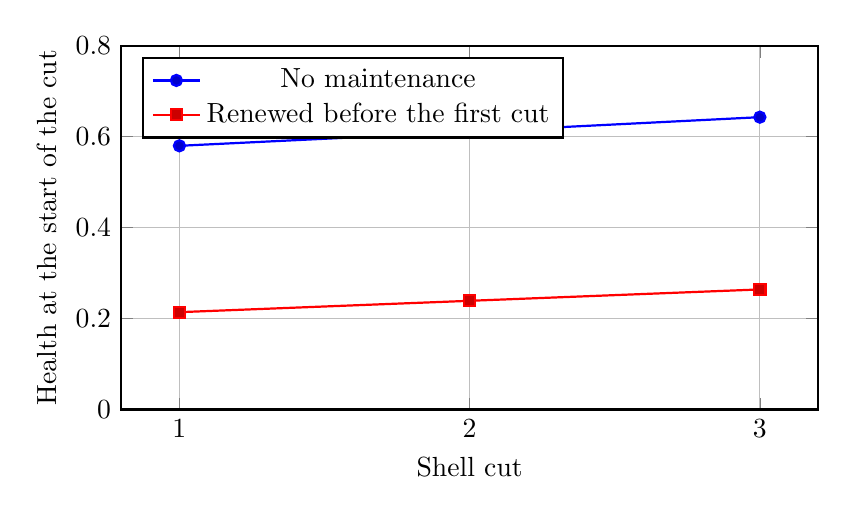
\begin{tikzpicture}
\begin{axis}[
  width=0.86\textwidth,
  height=6.2cm,
  xlabel={Shell cut},
  ylabel={Health at the start of the cut},
  xmin=0.8, xmax=3.2,
  ymin=0, ymax=0.8,
  xtick={1,2,3},
  grid=both,
  legend pos=north west,
  thick
]
\addplot coordinates {(1,0.580) (2,0.611) (3,0.643)};
\addlegendentry{No maintenance}
\addplot coordinates {(1,0.214) (2,0.239) (3,0.264)};
\addlegendentry{Renewed before the first cut}
\end{axis}
\end{tikzpicture}
\caption{Health of Cutter-A at the start of three identical shell cuts. The renewed path begins after Equation~\eqref{eq:pm-map}. Neither path is a failure time. Both are the state the next score will read.}
\label{fig:threeh}
\end{figure}

The energy accounting moves the same way and is easier to underestimate. The unrepaired first cycle draws about \(3.90\,\mathrm{kWh}\) plus a share of the repair. The repaired first cycle draws \(4.65\,\mathrm{kWh}\) because the maintenance minutes are charged. By the third cycle the unrepaired cutter is both slower and hotter, and the nameplate \(6.8\,\mathrm{kW}\) is multiplied by a larger health surcharge. The day-level energy gaps in Chapter~\ref{ch:estimation}, on the order of \(100\,\mathrm{kWh}\), are this third-cycle effect summed over every occupation, not a property of one row of Table~\ref{tab:worked}.

\subsection{How many decisions a day contains}

A book of sixteen orders has, on the routes of Section~\ref{sec:problem-set}, somewhere between six and eight operations each, so the cell starts on the order of one hundred and twenty bundles. Each bundle is one call to the scorer. At a typical call the feasible set is not one hundred and twenty. Precedence keeps only the next operation of each released order, and capacity keeps only the free machines and free operators. A call with eight ready operations, two legal machines, and two legal operators is a few dozen scores, each a constant-time evaluation of Equations~\eqref{eq:raw1}--\eqref{eq:psi} and, when the twin is on, Algorithm~\ref{alg:ssdt}. The day is a few thousand such scores. That is why identification, which repeats the day a few thousand times, finishes as a batch job, and why dispatch, which does it once, is not the thing a planner waits for.

The multi-layer model changes the constant, not the number of decisions. Each layer costs a pass over the edges of the candidate graph. Four nodes and a handful of typed edges remain a small graph. The reason to defer that model is not computer time. It is the absence, in this thesis, of a plant large enough for the hand-grouped keys to be the wrong inductive bias. Twenty identified coefficients already expose which costs matter. A deeper network would hide that exposure unless its attention weights were read back out, which is possible and was not necessary here.

The evolutionary reference pays a different bill. A population of eighteen, decoded twelve times and then doubled inside the generational pool, is a few hundred full days of simulation for one book, and it returns a front for that book only. Repeating it at every rush release is the cost Section~\ref{sec:tech1-review} objected to. The online score pays the identification once and then pays one argmin per free resource.

\subsection{Where the disjunctive graph went}

It is reasonable to ask whether the four-node candidate graph replaced the disjunctive graph or merely decorated it. Precedence is still a chain of conjunctive arcs: an operation enters \(R(t)\) only when its predecessor has finished. Machine capacity is still disjunctive: two bundles share a machine only in sequence, because a busy machine is not in \(\mathcal{F}\). The same sentence holds for an operator. The token inequality \eqref{eq:token} has no classical disjunctive counterpart, because a die is not a machine and two operations can hold two dies at the same time. The candidate graph is the disjunctive graph at the moment a decision is taken, restricted to the operations that could actually start, and extended by the operator and the shop node.

What was given up is an explicit binary \(y_{aa'}\) for every pair of operations that might ever conflict. Those binaries are the right variables for a solver that wants a certificate of optimality on a frozen instance. They are the wrong variables for a policy that must act when the instance is not frozen. Proposition~\ref{prop:mask} is the certificate this construction offers instead: every executed bundle was feasible when it started, and every operation eventually starts. It is not a certificate that no other feasible schedule has a smaller \(J_\omega\). The thesis does not claim that certificate. The tables measure the distance to four rules and to two ablations, which is a different and, for a running cell, a more relevant distance.

\subsection{A sensor reading, worked as a Kalman step}

The estimation plant writes health with Equation~\eqref{eq:plant-wear} and never opens Equation~\eqref{eq:kalman-upd}. This subsection runs the filter once, on the same cutter, so the sensor path is not only a citation. Take the posterior before a shell cut to be \(\hat h = 0.58\) with variance \(v = 0.010\). The drift is the cutter's own \(\eta = 0.00115\) per minute. The diffusion scale is taken as \(\sigma = 0.015\) per square-root minute, a design value for the indicator noise, not a fitted plant parameter. The cycle length is the unrepaired \(p = 27.268\) minutes.

Predict:
\begin{equation}
\hat h^{-} = 0.58 + 0.00115 \times 27.268 = 0.6114 ,
\end{equation}
\begin{equation}
v^{-} = 0.010 + (0.015)^2 \times 27.268 = 0.01614 .
\end{equation}
Suppose the indicator, after the feature map, reads \(y = 0.64\), a little worse than the drift expected, with noise variance \(\rho^2 = 0.008\). The gain and the update are
\begin{equation}
K = \frac{0.01614}{0.01614 + 0.008} = 0.6685 ,
\end{equation}
\begin{equation}
\hat h = 0.6114 + 0.6685 \times (0.64 - 0.6114) = 0.6305 ,
\end{equation}
\begin{equation}
v = (1 - 0.6685) \times 0.01614 = 0.00535 .
\end{equation}
The reading moved the state from the pure-drift value \(0.611\) to \(0.631\), and it cut the variance. A second reading will move it less, because \(v\) is now smaller and the gain will fall. That is the filter doing the job Gebraeel and co-authors asked of a Bayesian residual: one bad minute does not become the new truth, and a persistent bias does not stay outside the state \cite{gebraeel2005}.

Now apply the Gaussian ceiling \eqref{eq:gauss-threshold} at \(\varepsilon = 0.10\), so \(\Phi^{-1}(0.90) \approx 1.282\), with ceiling \(h^{\star} = 0.90\), to the question ``may this same cycle be repeated.'' Using the updated health,
\begin{equation}
0.6305 + 0.00115 \times 27.268 + 0.015 \sqrt{27.268} \times 1.282 = 0.762 .
\end{equation}
The value \(0.762\) is under \(0.90\). The Gaussian one-step ceiling would allow another cycle. The hazard \eqref{eq:phi} at health \(0.6305\) and the same cycle length is \(0.144\), which is above \(\varepsilon = 0.10\). Algorithm~\ref{alg:ssdt} would veto. The two forms, which Section~\ref{sec:ssdt} presented as the same kind of object, disagree on this borderline cycle.

The disagreement is useful and it is not a bug in the arithmetic. Equation~\eqref{eq:gauss-threshold} asks whether the health at the end of the cycle is likely to have crossed \(0.90\). Equation~\eqref{eq:phi} asks whether an interruption intensity, which turns on at \(0.40\), has accumulated enough hazard to exceed the tolerance. A machine can be likely to survive the cycle without hitting \(0.90\) and still be likely enough to suffer a stop that the factory does not want. The estimation uses the hazard, because the cell's interruption model is an intensity, not a first hitting time of \(0.90\). A plant whose maintenance standard is literally ``stop at indicator \(0.90\)'' should use the Gaussian ceiling instead, and should expect fewer vetoes on this cutter. Publishing both formulas, and one numerical case where they split, is what makes the tolerance a parameter rather than a story.

The variance also says when the filter is not yet allowed to veto. At the start of a shift, if \(v\) is large, \(K\) is near one and a single noisy \(y\) can throw \(\hat h\) across \(\varepsilon\). The practical rule is to withhold Algorithm~\ref{alg:ssdt} until \(v\) has fallen below a band, or to inflate \(\varepsilon\) by a term in \(\sqrt{v}\). Neither guard is in the estimation, because the plant variance is zero. Both belong in the specification for a cutter whose indicator is new.

\subsection{What Chapter~\ref{ch:estimation} is allowed to claim about these formulas}

\subsection{Failure modes of the score}

The score can be wrong in ways the mask will not catch, because the mask only enforces feasibility. Four failure modes are worth naming before the estimation, so that a bad table can be traced to a cause.

The first is a stale divisor. If batch quantities move from around eighty to around twenty, \(\rho_1 = p/45\) becomes a small number for every candidate and the processing-time weight stops discriminating. The policy then leans on whatever cost is still order-one, which on this vector is load deviation. The shop will look balanced and late. The fix is to re-identify, not to edit \(5.660\) by hand.

The second is a health indicator that saturates. If every machine reports \(h\) near one because the feature map was fit on a different tool, then \(\rho_5\) and \(\rho_8\) are large for every candidate and the maintenance test fires on every cycle. The day fills with sixteen-minute renewals that do not change a saturated indicator, because Equation~\eqref{eq:pm-map} pulls \(h\) down and the next reading, if it is still saturated, puts it back. The twin then oscillates. The fix is the feature map, upstream of the scheduler.

The third is an opening that was identified at one preference and then used at another. Section~\ref{sec:rch} already recorded that the shop-node opening at the balanced \(\omega\) is negative and nearly silent. Feeding an energy-heavy \(\omega\) through Equations~\eqref{eq:open-op}--\eqref{eq:open-s} without a new identification does not create an energy policy. It rescales a policy that was fit to balance load. Chapter~\ref{ch:estimation} therefore does not draw a Pareto front from those openings.

The fourth is a token capacity of zero that the data claim is one. The mask will refuse every operation of that colour, the clock will advance only when some other colour can run, and an order of the missing colour will wait until the end and then, if no other work remains, deadlock is avoided only because capacity one was assumed in Proposition~\ref{prop:mask}. A capacity of zero violates the hypothesis of the proposition. The cell should reject such a book at load time rather than discover it as a stuck clock.

None of these modes appeared in the estimation books, because the divisors match the batch sizes, the health values start inside \((0,1)\) and move by the wear recursion rather than by a saturated sensor, the preference is the one that was identified, and every token pool has capacity at least one. They are listed because a transfer of the same code to a different bag line will hit them in that order.

\begin{table}[ht]
\centering
\caption{What to check when a transferred cell misbehaves. The estimation books did not trip these checks.}
\label{tab:failmodes}
\small
\begin{tabular}{llp{6.2cm}}
\toprule
Symptom & Likely cause & Check \\
\midrule
Balanced and late & stale time divisor & re-identify after rescaling \(\rho_1\) \\
Maintenance every cycle & saturated health & inspect the feature map, not \(\varepsilon\) \\
Energy weight ignored & old \(\omega\) in the openings & rerun Algorithm~\ref{alg:cem} \\
Clock stuck on one colour & token capacity zero & reject the book before dispatch \\
\bottomrule
\end{tabular}
\end{table}

An implementation that follows this chapter, rather than the estimation program, has a definite order of work. First the routes, the skill matrix, the token capacities, and the nameplate powers are tables, not code. Second the mask is written and tested on a first-in-first-out ranking, because Proposition~\ref{prop:mask} can be checked before any weight exists: every order must finish, and no token count may go negative. Third the twelve raw costs are logged for a single candidate and checked against a hand calculation of the kind in the cutter example. Fourth the weights are identified, and the log-weights are inspected. A colour weight near zero, as in Equation~\eqref{eq:wstar}, is a result to be reported, not a bug to be patched by hand. Fifth the maintenance test is switched on at a stated \(\varepsilon\), and a one-machine trace like Table~\ref{tab:threecycle} is checked before any full book is compared. Sixth, and only if a sensor exists, the Kalman step is put in front of the wear recursion and the variance guard is set so that a new indicator cannot veto on its first noisy hour. Skipping to a multi-layer network at step two would make every later check harder and would not change the mask.

The two technologies, stripped of the surrounding discussion, are small enough to restate. RCH-GAT builds, at each free resource, the feasible bundles of Equation~\eqref{eq:bundle}, scores them by the preference-weighted attention of Equation~\eqref{eq:psi}, and starts the minimiser. The graph has four node types because the bundle names an operation, a machine, an operator, and a token. The weights in Equation~\eqref{eq:wstar} say which of those nodes the identification actually used: load, skill, failure, setup, and energy, with colour contention nearly silent. SSDT-CC writes the health that those failure and energy costs read. It lengthens processing time by Equation~\eqref{eq:ptime}, assigns an interruption probability by Equation~\eqref{eq:phi}, and, when that probability exceeds \(\varepsilon\) or the predicted health exceeds \(0.90\), renews the machine by Equation~\eqref{eq:pm-map} before the cycle. The renewal is not free on the cycle that pays it. Three cycles later, on the numbers of Table~\ref{tab:threecycle}, it is cheaper than letting the cutter drift. A sensor path, when one exists, revises the same health by Equations~\eqref{eq:kalman-pred} and \eqref{eq:kalman-upd}, and it can disagree with the hazard on a borderline cycle, as the numerical Kalman step showed. The estimation is allowed to speak only for the subset it ran.

The formulas of this chapter define the system. The next chapter measures an executable subset of them on a simulated school-bag cell. The subset includes Equations~\eqref{eq:ptime}, \eqref{eq:raw1}--\eqref{eq:psi}, \eqref{eq:phi}, \eqref{eq:pm-map}, and Algorithms~\ref{alg:cem}--\ref{alg:ssdt}. The subset does not include a trained multi-layer network \eqref{eq:gat-full}--\eqref{eq:gat-update} and does not include a noisy sensor around \eqref{eq:kalman-upd}. Claims about makespan, energy, and failures in the next chapter are claims about the subset. Claims about the multi-layer network and the Kalman filter are claims about the model that the subset instantiates, and they are not given extra experimental authority.
